\documentclass[twoside,11pt,openright]{report}

\usepackage[utf8x]{inputenc}
\usepackage[american]{babel}
\usepackage{a4}
\usepackage{latexsym}
\usepackage{amssymb}
\usepackage{amsmath}
\usepackage{amsthm}
\usepackage{epsfig}
\usepackage[T1]{fontenc}
\usepackage{mathptmx}
\usepackage{color}
\usepackage{epstopdf}
\usepackage{microtype}
\usepackage{hyperref}
\usepackage{algorithm}
\usepackage[noend]{algpseudocode}
\usepackage[useregional]{datetime2}
\DTMlangsetup[en-US]{showdayofmonth=false}
\usepackage{lipsum}
% \usepackage{pmboxdraw}
\usepackage{textgreek}
\usepackage[dvipsnames]{xcolor}
\usepackage[outputdir=build]{minted}
\setminted{fontsize=\footnotesize}
\usepackage{tikz}
\usepackage{float}
\usepackage{graphicx}
\usepackage{subcaption}
\usepackage{caption}
\usepackage{geometry}

\theoremstyle{definition}
\newtheorem{exmp}{Example}[chapter]

\renewcommand*\sfdefault{lmss}
\renewcommand*\ttdefault{txtt}

\newcommand{\todo}[1]{{\color[rgb]{.5,0,0}\textbf{$\blacktriangleright$#1$\blacktriangleleft$}}}

\begin{document}

%%%%%%%%%%%%%%%%%%%%%%%%%%%%%%%%%%%%%%%%%%%%%%%%%%%%%%%%%%%%%%%%%%%%%%%

\pagestyle{empty}
\pagenumbering{roman}
\vspace*{\fill}
\noindent{\rule{\linewidth}{1mm}\\[4ex]
{\Huge\sf Improving Performance of the Datalog Engine in Flix}\\[2ex]
{\huge\sf Zijun Yu, 202203581}\\[2ex]
\noindent\rule{\linewidth}{1mm}\\[4ex]
\noindent{\Large\sf Master's Thesis, Computer Science\\[1ex]
  \today \\[1ex] Advisor: Magnus Madsen\\[15ex]}\\[\fill]}

\epsfig{file=logo.eps}
\clearpage

%%%%%%%%%%%%%%%%%%%%%%%%%%%%%%%%%%%%%%%%%%%%%%%%%%%%%%%%%%%%%%%%%%%%%%%

\pagestyle{plain}
\chapter*{Abstract}
\addcontentsline{toc}{chapter}{Abstract}

% \lipsum[1] % Placeholder for the abstract text.

% \chapter*{Resumé}
% \addcontentsline{toc}{chapter}{Resumé}

% \todo{in Danish\dots}

\chapter*{Acknowledgments}
\addcontentsline{toc}{chapter}{Acknowledgments}

\todo{Write acknowledgments here\dots}

\vspace{2ex}
\begin{flushright}
  \emph{Zijun Yu,}\\
  \emph{Aarhus, \today.}
\end{flushright}

\tableofcontents
\cleardoublepage
\pagenumbering{arabic}
\setcounter{secnumdepth}{2}

%%%%%%%%%%%%%%%%%%%%%%%%%%%%%%%%%%%%%%%%%%%%%%%%%%%%%%%%%%%%%%%%%%%%%%%

\chapter{Introduction}
\label{ch:intro}

Datalog is a simple yet powerful declarative logic programming language. Programs written in a logic programming language are collections of logical statements and rules. This allows the programmer to solve problems by stating facts and rules about the problem domain rather than by giving step-by-step algorithmic instructions.

The Flix programming language is a new functional, declarative, and strongly typed programming language on the JVM. One of its main features is the first-class support for Datalog, allowing programmers to write Datalog programs directly in Flix.

The Datalog engine in Flix is implemented as a library using semi-naïve evaluation as its evaluation strategy, as most modern Datalog engines do. The Datalog engine in Flix has two parts: it compiles the given Datalog program into an intermediate representation, RAM (Relational Algebra Machine), represented as Flix values, and then it interprets the RAM program statement by statement. The semi-naïve evaluation is reflected in the way the RAM program is constructed. The generated RAM program is highly parallelizable, but it requires a concurrent data structure.

The goal of this thesis is to improve the performance of the Datalog engine in Flix. The main contribution of this thesis is the parallelization of the evaluation, which includes three parts: (1) a benchmark suite is proposed for evaluating the performance of the engine, (2) a new parallel statement is added to RAM, and (3) a concurrent data structure is implemented to enable the interpretation of the parallel statement. Specifically, a concurrent B+-tree is implemented to replace the Red-black tree used in the current implementation. The thesis statement is as follows: A concurrent B+-tree would make Datalog evaluation in Flix more efficient.

The rest of the thesis is organized as follows. In Chapter~\ref{ch:background}, we give a brief introduction to Datalog, including the syntax and semantics of the language, as well as the semi-naïve evaluation and how it leads to parallelism. In Chapter~\ref{ch:datalog_evaluation}, we first look at how the semi-naïve algorithm is implemented in Flix, specifically how the RAM program is constructed and interpreted. We then examine how parallelism can be introduced. Lastly, we discuss the benchmark suite. In Chapter~\ref{ch:btrees}, we look at the concurrent B+-tree implementation. In Chapter~\ref{ch:evaluation}, we evaluate the performance of the new implementation.

%%%%%%%%%%%%%%%%%%%%%%%%%%%%%%%%%%%%%%%%%%%%%%%%%%%%%%%%%%%%%%%%%%%%%%%

\chapter{Datalog}
\label{ch:datalog}

\section{Datalog Syntax}

A Datalog program consists of \textit{facts}, which are statements that are held to be true, and \textit{rules}, which describe how to deduce new facts from known facts. One can think of facts as rows in a relational database table and rules as queries that can be run on the database or views that can be materialized.

\begin{exmp}
  The following database stores the edges of a directed graph by means of facts of the form
  \texttt{edge(v1, v2)}, meaning that there is an edge from vertex \texttt{v1} to vertex \texttt{v2} in the graph:
  \begin{minted}{text}
    edge("a", "b").
    edge("b", "c").
    edge("c", "d").
  \end{minted}
  Below are two rules to compute the transitive closure of a graph stored by means of \texttt{edge} facts:
  \begin{minted}{text}
    tc(X, Y) :- edge(X, Y).
    tc(X, Y) :- edge(X, Z), tc(Z, Y).
  \end{minted}
  Intuitively, the first rule above says that if there is an edge from vertex \texttt{X} to vertex \texttt{Y}, then \texttt{(X, Y)} belongs to the transitive closure of the graph. The second rule says that if there is an edge from \texttt{X} to \texttt{Z} and there exists a vertex \texttt{Y} such that \texttt{(Z, Y)} belongs to the transitive closure, then \texttt{(X, Y)} belongs to the transitive closure as well.
\end{exmp}
\label{exmp:tc}

We now give the formal syntax of Datalog programs. A \textit{Datalog rule} $r$ is of the form:
$$A_0 :- A_1, \ldots, A_n.$$
where $n \geq 0$, the $A_i$'s are \textit{atoms}, and every atom is of the form $p(t_1, \ldots, t_m)$, where $p$ is a \textit{predicate symbol} and the $t_i$'s are \textit{terms}. A \textit{term} is either a \textit{variable} or a \textit{constant}. In the example above, \texttt{edge} and \texttt{tc} are predicate symbols, \texttt{"a"}, \texttt{"b"}, \texttt{"c"}, \texttt{"d"} are constants, and \texttt{X}, \texttt{Y}, \texttt{Z} are variables. Every variable appearing in $A_0$ (the \textit{head} of a rule) also appears in at least one of the $A_1, \ldots, A_n$ (the \textit{body} of a rule). This requirement is called \textit{safety} and is used to avoid rules yielding infinite sets of facts from a finite set of facts. The intuitive meaning of the Datalog rule above is that if the atoms $A_1, \ldots, A_n$ are true, then the atom $A_0$ is also true. A \textit{fact} is a rule with an empty body, i.e., a rule of the form $A_0 :-.$ which can be written as $A_0.$.

A \textit{Datalog program} is a finite set of Datalog rules. The \textit{definition} of a predicate symbol $p$ in a program $P$, denoted $def(p, P)$, is the set of rules of $P$ having $p$ in the head atom. Recall that a database can be seen as a finite set of facts. In the context of logic programming, all the knowledge (facts and general rules) is usually contained in a single logic program. We consider two sets of Datalog rules:
\begin{enumerate}
  \item A set of facts $D$ that represent tuples (rows) of a database.
  \item A Datalog program $P$ whose rules define new relations (or "views") from the database.
\end{enumerate}
$D$ is called the \textit{Extensional Database} (EDB) and $P$ is called the \textit{Intensional Database} (IDB). We will refer to $D$ as the database and $P$ as the Datalog program. Thus, predicate symbols are partitioned into two disjoint sets: \textit{base} (or EDB or \textit{extensional}) and \textit{derived} (or IDB or \textit{intensional}). The definition of base predicate symbols is stored in $D$. Base predicate symbols can appear in the body of rules in $P$ but not in the head. Derived predicate symbols cannot appear in $D$ and their definition is in $P$. We will use $P_D$ to denote $P \cup D$.

\section{Datalog Semantics}

We give the least-fixpoint semantics of Datalog, which defines the outcome of the program in an operational way, based on repeatedly applying the rules of the program until no new facts can be derived and thus a fixpoint is reached. It is well known that this semantics is equivalent to the model-theoretic semantics as well as the proof-theoretic semantics \cite{10.5555/551350}.

The fixpoint semantics is given in terms of an operator called the \textit{immediate consequence operator}, which derives new ground atoms starting from known ground atoms, using the rules of the program. Namely, $T_{P_D}$ takes as input a set of ground atoms $I$, applies the rules, and returns as output a set of ground atoms $T_{P_D}(I)$, called the \textit{immediate consequences} of $I$ w.r.t. $P_D$. We say that a set of ground atoms $I$ is a \textit{fixpoint} of $T_{P_D}$ if $T_{P_D}(I) = I$.

It is easy to see that $T_{P_D}$ is monotonic, that is, if $I_1 \subseteq I_2$, then $T_{P_D}(I_1) \subseteq T_{P_D}(I_2)$ for any sets of ground atoms $I_1$ and $I_2$. By the Knaster-Tarski theorem, since $T_{P_D}$ is monotonic, it has a least fixpoint (that is, a fixpoint that is included in any other fixpoint), which we denote as $\textit{lfp}(T_{P_D})$. The fixpoint semantics of $P_D$ is given by the least fixpoint $\textit{lfp}(T_{P_D})$.

\begin{exmp}
  Consider the Datalog program in Example \ref{exmp:tc}. Applying $T_{P_D}$ yields the following:
  \begin{align*}
    I_1 = T_{P_D}(\emptyset) & = \{edge("a", "b"), edge("b", "c"), edge("c", "d")\},    \\
    I_2 = T_{P_D}(I_1)       & = I_1 \cup \{tc("a", "b"), tc("b", "c"), tc("c", "d")\}, \\
    I_3 = T_{P_D}(I_2)       & = I_2 \cup \{tc("a", "c"), tc("b", "d")\},               \\
    I_4 = T_{P_D}(I_3)       & = I_3 \cup \{tc("a", "d")\},                             \\
    I_5 = T_{P_D}(I_4)       & = I_4.
  \end{align*}
  Thus, $I_4$ is the least fixpoint of $T_{P_D}$.
\end{exmp}
\label{exmp:tpd}

\section{Datalog Evaluation}

The fixpoint semantics immediately leads to an algorithm to evaluate Datalog programs, called \textit{naïve evaluation}. To define the algorithm, we first define a function called \textit{Eval-Rule} that takes as input a rule $r$ and a set of ground atoms $I$ containing the relations of the predicates appearing in the body of the rule, and returns the set of ground atoms that are the immediate consequences of $I$ w.r.t. $r$. The function \textit{Eval-Rule} can be defined precisely using relational algebra, but we omit the details here, as the intuition is simple and clear.

\begin{exmp}
  Let $r$ be the second rule in Example \ref{exmp:tc} and $I = I_3$ in Example \ref{exmp:tpd}, calling \textit{Eval-Rule} on rule $r$ and relations \texttt{edge} and \texttt{tc} yields the following:
  $$
    \textit{Eval-Rule}(r, edge, tc) = \{tc("a", "c"), tc("b", "d"), tc("a", "d")\}.
  $$
\end{exmp}
\label{exmp:eval-rule}

We then define another function called \textit{Eval} that evaluates a set of rules whose predicates in the head are the same. Consider a program $P$ and a database $D$. Let $R_1, \ldots, R_n$ be the base relations and $P_1, \ldots, P_m$ be the derived relations. For each derived predicate symbol $p_i$, we define \textit{Eval}($p_i, R_1, \ldots, R_n, P_1, \ldots, P_m$) as the union of calling \textit{Eval-Rule} over all rules with $p_i$ in the head.

Now, given a Datalog program $P$ and a database $D$, where the base predicate symbols are $r_1, \ldots, r_n$, the derived predicate symbols are $p_1, \ldots, p_m$, and the base relations are $R_1, \ldots, R_n$, Algorithm \ref{alg:naive-eval} performs the evaluation of $P$ over $D$.

\begin{algorithm}
  \caption{Naïve Evaluation}
  \begin{algorithmic}[1] % The number in square brackets specifies the line numbering
    \For{$i \leftarrow 1$ to $m$}
    \State $P_i \leftarrow  \emptyset$
    \EndFor
    \Repeat
    \For{$i \leftarrow  1$ to $m$}
    \State $P'_i \leftarrow  P_i$
    \EndFor
    \For{$i \leftarrow  1$ to $m$}
    \State $P_i \leftarrow  \text{Eval}(p_i, R_1, \ldots, R_k, P'_1, \ldots, P'_m)$
    \EndFor
    \Until{$P_i = P'_i$ for all $1 \leq i \leq m$}
    \State \Return $P_1, \ldots, P_m$
  \end{algorithmic}
\end{algorithm}
\label{alg:naive-eval}

One shortcoming of the naïve evaluation is that in each iteration, all tuples computed in the previous iterations are recomputed. For example, in Example \ref{exmp:eval-rule}, the tuples \texttt{tc("a", "c")} and \texttt{tc("b", "d")} are already computed in the previous iteration (they are already in $I_3$). The problem is that in the naïve evaluation, in each iteration, the tuples of the derived relations from earlier iterations are used in \textit{Eval-Rule}. The solution to this problem is called \textit{semi-naïve evaluation}.

We start by introducing an incremental version of the \textit{Eval-Rule} function. Consider a rule $r$ of the form
$$A_0 :- A_1, \ldots, A_n.$$
and assume to have a relation $R_i$ and an “incremental” relation $\Delta R_i$ for each atom $A_i$ in the body of the rule. We define the incremental version of \textit{Eval-Rule} as follows:
\begin{equation*}
  \begin{split}
    \textit{Eval-Rule-Incr}(r, R_1, \ldots, R_n,  \Delta R_1, \ldots, \Delta R_n) = \\
    \bigcup_{1 \leq i \leq n} \textit{Eval-Rule}(r, R_1, \ldots, R_{i-1}, \Delta R_i, R_{i+1}, \ldots, R_n).
  \end{split}
\end{equation*}
We can now define the \textit{semi-naïve evaluation} as shown in Algorithm \ref{alg:semi-naive-eval}.

\begin{algorithm}
  \caption{Semi-naïve Evaluation}
  \begin{algorithmic}[1]
    \For{$i \leftarrow 1$ \textbf{to} $m$}
    \State $\Delta P_i \leftarrow \text{Eval-rule}(p_i, R_1, \ldots, R_k, \emptyset, \ldots, \emptyset)$
    \State $P_i \leftarrow \Delta P_i$
    \EndFor
    \Repeat
    \For{$i \leftarrow 1$ \textbf{to} $m$}
    \State $\Delta P'_i \leftarrow \Delta P_i$
    \EndFor
    \For{$i \leftarrow 1$ \textbf{to} $m$}
    \State $\Delta P_i \leftarrow \text{Eval-rule-incr}(p_i, R_1, \ldots, R_k, P_1, \ldots, P_m, \Delta P'_1, \ldots, \Delta P'_m)$
    \State $\Delta P_i \leftarrow \Delta P_i - P_i$
    \EndFor
    \For{$i \leftarrow 1$ \textbf{to} $m$}
    \State $P_i \leftarrow P_i \cup \Delta P_i$
    \EndFor
    \Until{$\Delta P_i = \emptyset$ \textbf{for all} $1 \leq i \leq m$}
    \State \Return $P_1, \ldots, P_m$
  \end{algorithmic}
\end{algorithm}
\label{alg:semi-naive-eval}

It is obvious that the semi-naïve evaluation is parallelizable. There are two levels of parallelism in Algorithm \ref{alg:semi-naive-eval}. First, each invocation of \textit{Eval-Rule-Incr} can be done in parallel, that is, the body of the loop from line 9 to line 12. Second, as per the definition of \textit{Eval-Rule-Incr}, the invocations of \textit{Eval-Rule} called by \textit{Eval-Rule-Incr} can also be done in parallel. This is the main idea of the parallelization of this thesis. Also, the body of the loop from line 1 to line 4 can be done in parallel.

\section{Datalog Extensions and Datalog in Flix}

%%%%%%%%%%%%%%%%%%%%%%%%%%%%%%%%%%%%%%%%%%%%%%%%%%%%%%%%%%%%%%%%%%%%%%%

\chapter{Datalog Evaluation in Flix}
\label{ch:datalog_evaluation}

In Flix, the Datalog engine is implemented as a library. When a Flix program is executed, the Datalog rules are compiled into an intermediate representation called RAM (Relational Algebra Machine), which is then interpreted statement by statement. The RAM program is constructed in a way that reflects the semi-naïve evaluation algorithm. In this chapter, we first look at how the semi-naïve algorithm is implemented in Flix, specifically how the RAM program is constructed and interpreted. We then examine how parallelism can be introduced. Lastly, we discuss the benchmark suite.

\section{RAM}

We will not introduce the definition of RAM as Flix code here. Instead, we will give examples of stringified RAM programs. We will denote $P_i, \Delta P_i, \Delta P_i'$ in Algorithm \ref{alg:semi-naive-eval} as \textit{Full} relations, \textit{Delta} relations, and \textit{New} relations.

\begin{exmp}
  Consider the Datalog program in Example \ref{exmp:tc}. We have one base predicate \texttt{edge} and one derived predicate \texttt{tc}. The initialization part of the semi-naïve evaluation algorithm (lines 1 to 4) will be translated into the following RAM program:
  \begin{minted}[escapeinside=||]{text}
    // tc(x, y) :- edge(x, y).
    search 0$ |$\in$| edge do
        project (0$[0], 0$[1]) into Δtc
    end;
    // tc(x, z) :- tc(x, y), edge(y, z).
    search 0$ |$\in$| tc do
        query {1$ |$\in$| edge |\textbar| 1$[0] == 0$[1]} do
            project (0$[0], 1$[1]) into Δtc
        end
    end;
    merge Δtc into tc;
  \end{minted}
  The invocation of \textit{Eval-Rule} for the derived predicate \texttt{tc} is translated into the above two RAM statements. The translation is on a rule-by-rule basis and is mechanical. Variables are represented by integers followed by a dollar sign and they hold a tuple of a relation. Each atom in the body is translated into a \textit{search}. The \textit{search} statement is used to iterate over the tuples of a relation. The \textit{query} statement is like \textit{search} but with a filter of the form \texttt{x[0]==a, x[1]==b, x[2]==c, ...}. The difference between using a \textit{query} and using a \textit{search} with \textit{if} conditions is that the former is more efficient, as the tuples are stored using trees and the query is interpreted using range queries on the trees that avoid unnecessary walking over the tree. We will see more about this in Chapter \ref{ch:btrees}.

  The main loop of the semi-naïve evaluation algorithm (lines 5 to 16) will be translated into the following RAM program:
  \begin{minted}[escapeinside=||]{text}
    until(Δtc == |$\emptyset$|) do
        purge Δtc';
        // tc(x, y) :- Edge(x, y).
        // tc(x, z) :- tc(x, y), Edge(y, z).
        search 0$ |$\in$| Δtc do
            query {1$ |$\in$| Edge |\textbar| 1$[0] == 0$[1]} do
                if((0$[0], 1$[1]) |$\notin$| tc) then
                    project (0$[0], 1$[1]) into Δtc'
                end
            end
        end;
        merge Δtc' into tc;
        Δtc := Δtc'
    end
  \end{minted}

  In this program, \texttt{tc} is the only derived predicate. Calling \textit{Eval-Rule-Incr} for \texttt{tc} includes the translation of both rules. However, there is no derived predicate in the body of the first rule, so the first rule is translated to an empty statement. For the second rule, the derived predicate \texttt{tc} appears in one atom in the body, so the \textit{search} statement is used to iterate over the \textit{New} relation $\Delta$\texttt{tc}. In Algorithm \ref{alg:semi-naive-eval}, line 11 is used to compute the \texttt{New} relations by set difference. In the implementation, it is done by the \textit{if} operation to check if the tuple is already in the \texttt{Full} relation.
\end{exmp}
\label{exmp:tc-ram}

We will show one more example of a more complex Datalog program, where derived predicates appear more than once in the body of a rule, which will make the translation of \textit{Eval-Rule-Incr} more interesting.

\begin{exmp}
  The following Datalog program performs a point-to analysis of variables in a C program \cite{PGL-014}. The instructions of the program can be translated into \textit{EDB} relations as follows:
  \begin{minted}[escapeinside=||]{text}
    AddressOf(a, b) |$\small \text{representing}$| a=\&b
    Assign(a, b) |$\small \text{representing}$| a=b
    Load(a, b) |$\small \text{representing}$| a=*b
    Store(a, b) |$\small \text{representing}$| *a=b
  \end{minted}
  The point-to analysis can now be done using a Datalog program storing pairs of variables \texttt{a} and \texttt{b} in the intentional relation \texttt{PointsTo} if \texttt{a} may point to \texttt{b}. The program contains the following four rules with the same head:
  \begin{minted}{text}
    PointsTo(x, y) :- AddressOf(x, y).
    PointsTo(x, y) :- Assign(x, z), PointsTo(z, y).
    PointsTo(x, w) :- Load(x, z), PointsTo(z, y), PointsTo(y, w).
    PointsTo(x, y) :- Store(z, w), PointsTo(z, x), PointsTo(w, y).
  \end{minted}
  We pay attention to the load rule (the third rule). \textit{Eval-Rule} (line 2 of Algorithm \ref{alg:semi-naive-eval}) for this rule will be translated into the following single RAM statement:
  \begin{minted}[escapeinside=||]{text}
    search 0$ |$\in$| Load do
        query {1$ |$\in$| PointsTo |$\textbar$| 1$[0] == 0$[1]} do
            query {2$ |$\in$| PointsTo |$\textbar$| 2$[0] == 1$[1]} do
                project (0$[0], 2$[1]) into ΔPointsTo
            end
        end
    end;
  \end{minted}
  Because there are two derived predicates in the body, \textit{Eval-Rule-Incr} (line 11 of Algorithm \ref{alg:semi-naive-eval}) for this rule will be translated into two RAM statements. This corresponds to the union operation in the definition of \textit{Eval-Rule-Incr}:
  \begin{minted}[escapeinside=||]{text}
    search 0$ |$\in$| Store do
        query {1$ |$\in$| ΔPointsTo |$\textbar$| 1$[0] == 0$[0]} do
            query {2$ |$\in$| PointsTo |$\textbar$| 2$[0] == 0$[1]} do
                if((1$[1], 2$[1]) |$\notin$| PointsTo) then
                    project (1$[1], 2$[1]) into ΔPointsTo'
                end
            end
        end
    end;
    search 0$ |$\in$| Store do
        query {1$ |$\in$| PointsTo |$\textbar$| 1$[0] == 0$[0]} do
            query {2$ |$\in$| ΔPointsTo |$\textbar$| 2$[0] == 0$[1]} do
                if((1$[1], 2$[1]) |$\notin$| PointsTo) then
                    project (1$[1], 2$[1]) into ΔPointsTo'
                end
            end
        end
    end;
  \end{minted}
\end{exmp}
\label{exmp:point-to}

\section{Parallelization}

It is now clear that each statement translated from a rule can be executed in parallel. Consider Example \ref{exmp:point-to}; the two \textit{search} statements in the \textit{Eval-Rule-Incr} for the load rule can be executed in parallel. In fact, the assign rule will be translated into one statement, the load rule and the store rule will both be translated into two statements. All five statements can be executed in parallel. We mentioned in the previous chapter that there are two levels of parallelism in the semi-naïve evaluation algorithm. This nested parallelism is automatically spread out in the way the RAM program is constructed.

The first thing to do is to add a new type of statement to RAM, called \texttt{Par} (Parallel), in contrast to the existing \texttt{Seq} (Sequential) statement:

\begin{minted}[escapeinside=||]{text}
  pub enum RamStmt[v] {
      case Insert(RelOp[v])
      case Merge(RamSym[v], RamSym[v])
      case Assign(RamSym[v], RamSym[v])
      case Purge(RamSym[v])
      case Seq(Vector[RamStmt[v]])
      |\textcolor{red}{case Par(Vector[RamStmt[v]])}|
      case Until(Vector[BoolExp[v]], RamStmt[v])
      ...
  }
\end{minted}

One thing to note is that in the previous text we refer to \texttt{search} and \texttt{query} as statements, whereas in the actual implementation they are cases of the \texttt{RelOp} enum, along with \texttt{If} and \texttt{Project}. All of them belong to the category of the \texttt{Insert} statement.

We then change the compiler to generate as many \texttt{Par} statements as possible. The new RAM program will be of the following form in general (we use \texttt{||} to denote parallel statements and \texttt{;} to denote sequential statements):

\begin{minted}[escapeinside=||]{text}
  search 0$ |$\in$| ... do
      ...
  end |\textcolor{red}{\textbar\textbar}|
  search 0$ |$\in$| ... do
      ...
  end |\textcolor{red}{\textbar\textbar}|
  ... |\textcolor{BlueGreen}{;}|
  merge Δ... into ... |\textcolor{red}{\textbar\textbar}|
  merge Δ... into ... |\textcolor{red}{\textbar\textbar}|
  ...                  |\textcolor{BlueGreen}{;}|
  Until ... do
      search 0$ |$\in$| ... do
          ...
      end |\textcolor{red}{\textbar\textbar}|
      search 0$ |$\in$| ... do
          ...
      end |\textcolor{red}{\textbar\textbar}|
      ... |\textcolor{BlueGreen}{;}|
      merge Δ...' into ... |\textcolor{red}{\textbar\textbar}|
      merge Δ...' into ... |\textcolor{red}{\textbar\textbar}|
      ...                   |\textcolor{BlueGreen}{;}|
      Δ... := Δ...' |\textcolor{red}{\textbar\textbar}|
      Δ... := Δ...' |\textcolor{red}{\textbar\textbar}|
      ...            |\textcolor{BlueGreen}{;}|
  end 
\end{minted}

When interpreting the RAM program, we will fire up one thread for each statement in a \texttt{Par} statement. The problem is then how to perform concurrent operations on the relations. We have mentioned that the tuples of a relation are stored using trees. More specifically, the tuples are stored in a red-black tree, where the keys are the tuples themselves, and the values are either \texttt{Unit} or the corresponding lattice value if lattice is used in the relation.

\section{Red-Black Trees}

After the parallelization, there will be more than one thread trying to insert tuples into the same relation, for instance, in Example \ref{exmp:point-to}. However, red-black trees do not support concurrent insertions. One naïve solution is to include a mutex lock in the red-black tree and change all insertion methods to acquire the lock at the beginning and release the lock at the end. This solution works but is not efficient, as usually, there is more than one rule for deriving a predicate in a realistic Datalog program, and the thread will be blocked by the lock. We will not demonstrate the evaluation of this solution in later sections, but we mention that it sees 1.0x - 1.2x speedup on the realistic tests in our benchmark.

In this section, we will give a brief introduction to red-black trees. More specifically, we will look at what range query is and how it has made Datalog evaluation more efficient.

A red-black tree is a specialized binary search tree data structure. Compared to other self-balancing binary search trees, the nodes in a red-black tree hold an extra bit called "color" representing "red" and "black," which is used when re-organizing the tree to ensure that it is always approximately balanced.

Binary search trees are used to store ordered data. In our case, the data is the tuples of a relation (serving as keys), possibly associated with a lattice value (serving as values). In a binary search tree, each node stores a key and a value, and the left child of a node has a key less than the node's key, and the right child has a key greater than the node's key. This sorted property allows for an efficient range query.

A range query is a query that retrieves data in a given range. In our case, the keys are tuples, and they are sorted first by the first element, then by the second element, and so on. As we have illustrated in Example \ref{exmp:tc-ram}, the \texttt{query} statement is always of the form \texttt{x[0]==a, x[1]==b, x[2]==c, ...}. When we are doing a range query, if at the current node, the first element of the key is less than \texttt{a}, or if the first element of the key is equal to \texttt{a} but the second element of the key is less than \texttt{b}, we can skip the left child of the current node, and so on. Likewise, we can skip the right child for some node. Only when the equality is met for all the elements in the query condition, we will visit both the left child and the right child.

\section{Benchmark}

We have implemented a small benchmark suite that contains four files, 13 programs in total, to evaluate the performance of the Datalog engine in Flix.
\begin{itemize}
  \item \texttt{Closure.flix} contains four realistic programs that compute either the transitive closure or something similar (e.g., strongly connected component) on graphs.
  \item \texttt{Pointer.flix} contains two programs that perform point-to analysis as shown in Example \ref{exmp:point-to}. The difference between the two programs is in the order of the variables in the rule. We will discuss this in Chapter \ref{ch:future_work}.
  \item \texttt{Intersect.flix} and \texttt{Propagate.flix} contain four and three programs respectively that are rather artificial. For example, the third program in \texttt{Propagate.flix} is as follows:
        \begin{minted}{text}
    pub def propaget3(): Int32 =
        let p = #{
            A(slowId(x) + 1) :- Z(x), A(x).
            B(slowId(x) + 1) :- Z(x), B(x).
            C(slowId(x) + 1) :- Z(x), C(x).
            ...
            Z(slowId(x) + 1) :- Z(x), if x < 6.
        };
        let f = #{
            Z(0).
            A(0).
            B(0).
            C(0).
            ...
        };
        query p, f select x from A(x)
        |> Vector.length
  \end{minted}
        \texttt{SlowId} is an identity function that takes a long time to compute by calling a recursive Fibonacci function inside. In the semi-naïve evaluation, each rule will produce a new one-element tuple for each relation, stopping at 6. Because we only have one rule for each predicate, adding parallelism should significantly speed up the evaluation, no matter using the naïve mutex lock solution or using an advanced concurrent tree. Indeed, when evaluating this program on a 14-core machine, we see a 6x speedup using the mutex lock solution.
\end{itemize}

%%%%%%%%%%%%%%%%%%%%%%%%%%%%%%%%%%%%%%%%%%%%%%%%%%%%%%%%%%%%%%%%%%%%%%%

\chapter{B-Trees}
\label{ch:btrees}

We have discussed in previous sections that the tuples of a relation are stored using red-black trees and we want to change to a concurrent data structure to facilitate parallelism. The new data structure should act like a set and support efficient range queries.

The B-tree and its variants are widely used and studied in database systems. Many papers have described how to perform concurrent operations on B-trees. In this section, we will give a brief introduction to B-trees and B+ trees, and then we will introduce a new variant of B-trees called $\text{B}^{\text{link}}$ trees that support concurrent reading and writing. In the next chapter, we will evaluate the performance of the Datalog engine using B+ trees and $\text{B}^{\text{link}}$ trees.

\section{B-Trees and B+ Trees}

The B-tree is a multi-way search tree. A $m$-way search tree is a tree where each node has at most $m$ children, hence storing at most $m-1$ keys. The keys in a node are sorted, and the keys in the children of a node are in the range defined by the keys of the node.

A B-tree of order m is a tree which satisfies the following properties:
\begin{itemize}
  \item Every node has at most $m$ children.
  \item Every node, except for the root and the leaves, has at least $\lceil m/2 \rceil$ children.
  \item The root node has at least two children unless it is a leaf.
  \item All leaves appear on the same level.
  \item A non-leaf node with k children contains $k-1$ keys.
\end{itemize}

In B-trees, every node stores a range of keys and their corresponding values. Each internal node's keys, including the root node, act as separation values which divide its subtrees, as shown in figure \ref{fig:btree_node} For example, if an internal node has 3 child nodes (or subtrees) then it must have 2 keys: $a_1$ and $a_2$. All values in the leftmost subtree will be less than $a_1$, all values in the middle subtree will be between $a_1$ and $a_2$, and all values in the rightmost subtree will be greater than $a_2$.

The fourth property means that B-tree is a balanced tree. The second property ensures that each node is at least half full. This implies that two half-full nodes can be joined to make a legal node, and one full node can be split into two legal nodes (with an element pulled out and put into the parent). This properties make it possible to delete and insert new values into a B-tree and adjust the tree to preserve the B-tree properties.

A B+ tree is a variant of a B-tree where the internal nodes do not store any pointers to records, thus all pointers to records are stored in the leaf nodes. In addition, a leaf node may include a pointer to the next leaf node to speed sequential access. This makes range queries easy to implement. Since in a B+ tree, values are not stored in internal nodes, all keys appear twice in the tree: once in an internal node and once in a leaf node. This leads to design choice to be made. In figure \ref{fig:btree_node}, if we denote all the keys stored in a subtree at pointer $P_i$ as $V_i$, then any $v \in V_i$ can either staisfy $K_{i-1} < v \leq K_i$ or $K_{i-1} \leq v < K_i$. We prefer the former because it makes the implementation of search consistent. When performing a search for some $k$ inside a node, we return the index of the first key that is greater than or equal to $k$. This index will always be the correct index of the pointer array to follow.

\begin{figure}[h]
  \centering
  \vspace{0.5em}
  \begin{tikzpicture}
    % Draw the main rectangle
    \draw (0,0) rectangle (8,0.8);

    % Draw the partitions
    \draw (1.2,0) -- (1.2,0.8);
    \draw (2.4,0) -- (2.4,0.8);
    \draw (3.6,0) -- (3.6,0.8);
    \draw (5.6,0) -- (5.6,0.8);
    \draw (6.8,0) -- (6.8,0.8);

    % Add labels inside the rectangles
    \node at (0.6,0.4) {\small $P_0$};
    \node at (1.8,0.4) {\small $K_1$};
    \node at (3.0,0.4) {\small $P_1$};
    \node at (4.6,0.4) {\small $\cdots$};
    \node at (6.2,0.4) {\small $K_{m}$};
    \node at (7.4,0.4) {\small $P_{m}$};

    % Draw arrows
    \draw[->] (0.6,0) -- (0.1,-0.8);
    \draw[->] (3.0,0) -- (3.0,-0.8);
    \draw[->] (7.4,0) -- (7.9,-0.8);
  \end{tikzpicture}
  \caption{A B+ tree node}
  \label{fig:btree_node}
\end{figure}


Compared to binary search trees, such as red-black trees, B-trees and its variants are more efficient in terms of I/O operations. B-trees are widely used in database systems to store indexes. The records in a database are stored in disk and pointers to the records are stored as values in the B-tree. The tree itself, serves as an index to the records, is also stored in disk. In our case, values are pointers to tuples in memory, and the tree is stored in memory as well. In binary search trees, there is a key and two pointers in each node, while in B-trees, $m$ keys are paired with only $m+1$ pointers. This means two things. First, since a key is paired with less pointers, B-trees use less memory. Second, the tree is shallower than a binary search tree so less pointers are followed to find a key. And since the keys are stored consecutively as an array in a node, the keys are more likely to be in the cache when search inside a node. This means that B-trees is more cache friendly than binary search trees.

Compared to B-trees, B+ trees have fewer pointers in the internal nodes. If we use a fixed size memory for a node, then B+ trees can hold more keys in one node, causing the tree to be shallower. And because we only store pointers to records in the leaf node, the structure of the leaf node is almost identical to the structure of the internal node. This also makes range query easier and efficient since we only need to traverse the leaf nodes and the leaf nodes are linked together. The definition of B+ tree in flix is as follows:

\begin{minted}{text}
 enum BPlusTree[k: Type, v: Type, r: Region](Region[r], Ref[Node[k, v, r], r])
 enum Node[k: Type, v: Type, r: Region] {
   case Inner(Ref[Int32, r], Array[k, r], Array[Node[k, v, r], r])
   case  Leaf(Ref[Int32, r], Array[k, r], Array[v, r], Ref[Node[k, v, r], r])
   case Empty
 }
\end{minted}

Flix is a functional-first programming language that encourages the use of immutable data structures, but it has rich support for imperative programming with destructive updates to mutable data. It uses its effect system to separate pure and impure code. In particular, It uses the region concept to track the use of mutable memory. In Flix, all mutable memory belongs to a region that is tied to its lexical scope. When execution leaves the lexical scope of a region, all memory in that region becomes unreachable.

Flix has two basic types of mutable memory: References and Arrays. Higher-level mutable data structures, such as the B+ tree here, are built on top of Refs and Arrays.

A B+ tree contains a region, which tracks the lifetime of the tree, and a reference to the root node of the tree. A region is needed because other mutable data, such as the nodes of the tree, should have the same lifetime as the tree, so they need to be allocated using the same region as the tree. Therefore, the constrcutor will take a region as an argument, as well as the configuration of the tree, i.e. how many children can a node have at most. A new tree can then be created as follows:

\begin{minted}{text}
def main(): Int32 =
  region r1 {
    let t = BPlusTree.empty(r1, 32);
    BPlusTree.size(t)
  }
\end{minted}

A node in the B+ tree can be either an inner node or a leaf node. The \texttt{Empty} case searves as \texttt{Null} in other languages. The structure of the inner node is similar to that of the leaf node, they both contain an array of keys, an array of child nodes or values respectively, and an integer that stores the number of keys that currently exist in the node. The leaf node contains an extra pointer to the right sibling.

\section{Insertion in B+ Trees}

We now give the insertion algorithm for a B+ tree in algorithm \ref{alg:bplus-insert}, which will be used in the evaluation in the next chapter and is also the base for the $\text{B}^{\text{link}}$ tree. For convenience, the variable $keys$ and $vals$ are used to represent the key and value arrays in the node that is currently examined in the context.

\begin{algorithm}[h]
  \caption{Insertion in B+ Tree}\label{alg:bplus-insert}
  \begin{algorithmic}[1] % The number in square brackets specifies the line numbering
    \Function{Insert}{$t, k, v$}
    \State $root \gets \text{root}(t)$
    \State $leaf, stack \gets \text{descendToLeaf}(root, k)$
    \State $i \gets \text{searchNode}(k, leaf)$
    \If {$i = \text{num}(keys)$ or $k \neq keys[i]$}
    \State \text{insertLeaf}$(k, v, i, stack, leaf, root)$
    \Else \State $keys[i] \gets k$
    \EndIf
    \EndFunction

    \Function{insertLeaf}{$k, v, i, node, stack, root$}
    \State $k', v' \gets$ insert $k$ and $v$ into $keys$ and $vals$
    \State \Comment {$k'$ and $v'$ are the overflowed key and value if the array is full}
    \If {$k'$ and $v'$ are null}
    \State increase the number of keys in the leaf by 1
    \Else
    \State $newNode, upKey \gets \text{splitLeaf}(node, k', v')$
    \State put $k'$ and $v'$ into $newNode$
    \If {$stack$ is empty}
    \State $newRoot \gets \text{create a new inner node}$
    \State put $upKey$, $leaf$, and $newNode$ in $newRoot$
    \State $root \gets newRoot$
    \Else
    \State $parent, i' \gets \text{pop}(stack)$
    \State insertInner($upKey$, $newNode$, $i'$, $parent$, $stack$, $root$)
    \EndIf
    \EndIf
    \EndFunction

    \Function{insertInner}{$k, n, i, node, stack, root$}
    \State same as insertLeaf, with the function of splitLeaf replaced by splitInner
    \EndFunction
  \end{algorithmic}
\end{algorithm}

The insertion algorithm is a recursive algorithm. It first descends to the leaf node where the key should be inserted. The descending function simply calls the search function to find the child node to follow and pushes the current node and the index of the child into a stack, and then repeatedly calls itself on the child node until it reaches a leaf node. The search function is a binary search function that returns the index of the first key that is greater than or equal to the key to be inserted, as we have discussed above.

The insertion function then checks if the key already exists in the leaf node, i.e. if the search reaches does not exceed the number of keys in the leaf node and the key is equal to the key at the index. If it exists, the value is updated. Otherwise, the key and value are inserted into the leaf node. The insertion may then cause the node to be split if the node is full. The split function will split the node into two nodes and return the key that should be inserted into the parent node. Recursive insertions are then performed using the stack. If we propagate all the way up util the stack is empty, then a new root node is created. There is one difference between splitting a leaf node and an inner node. As discussed, because values are only stored in leaf nodes in B+ trees, all keys appear twice in the tree. When splitting the leaf node, the middle key goes both into the new node and into the parent, while when splitting the inner node, the middle key leaves the current level and goes into the parent. This satisfy the sorted property ($K_{i-1} < v \leq K_i$) of the B+ tree.

\section{$\text{B}^{\text{link}}$ Trees}

There are many variants of B-trees that are designed to support concurrent reading and writing. In thisp roject, we mainly studied the $\text{B}^{\text{link}}$ tree proposed by Lehman and Yao \cite{10.1145/319628.319663}.

The idea of the $\text{B}^{\text{link}}$ is to add another key-pointer pair to each inner node and an additional key to each leaf node. The structure of a node in a $\text{B}^{\text{link}}$ tree is shown in figure \ref{fig:blink_node}. The additional key is called the \textit{high key}, i.e., the largest key in the subtree rooted at that node. For an inner node, the high key is the highest key in the subtree pointed by $P_m$. For a leaf node, the high key is the key is the same as $K_m$. The additional pointer is called \textit{link} and it points to the right sibling. The node on every level is now linked together, hence the name $\text{B}^{\text{link}}$ tree. Note this change still satisfy the sorted property of a node, that is, all keys in the subtree pointed by $P_m$ are greater than $K_m$ and less than or equal to the high key $K_{m+1}$.

\begin{figure}[h]
  \centering
  \vspace{0.5em}
  \begin{tikzpicture}
    % Draw the main rectangle
    \draw (0,0) rectangle (10.4,0.8);

    % Draw the partitions
    \draw (1.2,0) -- (1.2,0.8);
    \draw (2.4,0) -- (2.4,0.8);
    \draw (3.6,0) -- (3.6,0.8);
    \draw (5.6,0) -- (5.6,0.8);
    \draw (6.8,0) -- (6.8,0.8);
    \draw (8.0,0) -- (8.0,0.8);
    \draw (9.2,0) -- (9.2,0.8);

    % Add labels inside the rectangles
    \node at (0.6,0.4) {\small $P_0$};
    \node at (1.8,0.4) {\small $K_1$};
    \node at (3.0,0.4) {\small $P_1$};
    \node at (4.6,0.4) {\small $\cdots$};
    \node at (6.2,0.4) {\small $K_{m}$};
    \node at (7.4,0.4) {\small $P_{m}$};
    \node at (8.6,0.4) {\small $K_{m+1}$};
    \node at (9.8,0.4) {\small $P_{m+1}$};

    % Draw arrows
    \draw[->] (0.6,0) -- (0.1,-0.8);
    \draw[->] (3.0,0) -- (3.0,-0.8);
    \draw[->] (7.4,0) -- (7.9,-0.8);
    \draw[->] (10.4,0.4) -- (11.4,0.4); % Horizontal arrow to the right
  \end{tikzpicture}
  \caption{A $\text{B}^{\text{link}}$ tree node}
  \label{fig:blink_node}
\end{figure}

The $\text{B}^{\text{link}}$ tree is essentially a fine-grained locking scheme. Each node is paired with a lock. When a thread is accessing the fields in a node, it has to acquire the lock first. The high key and the link then serve as a way to know if the current node is being split by another thread. When accessing a node, if the search key  exceeds the high key, it means that the current node has been split and the thread should follow the link to the right sibling.

Figure \ref{fig:blink_tree} from Lehman and Yao shows an example of a $\text{B}^{\text{link}}$ tree. Our specification differs from Lehman and Yao in that the rightmost node at each level has $+\infty$ as its high value, i.e., all the 99's in the diagram are changed to $+\infty$. Although the key $+\infty$ never appears in the tree, this decision is consistent as long as in the begning when the empty root is created, $+\infty$ is set as the high value. We will see later that this will the implementation easier in section \ref{sec:blink-insert}.

\begin{figure}[h]
  \centering
  \vspace{0.5em}
  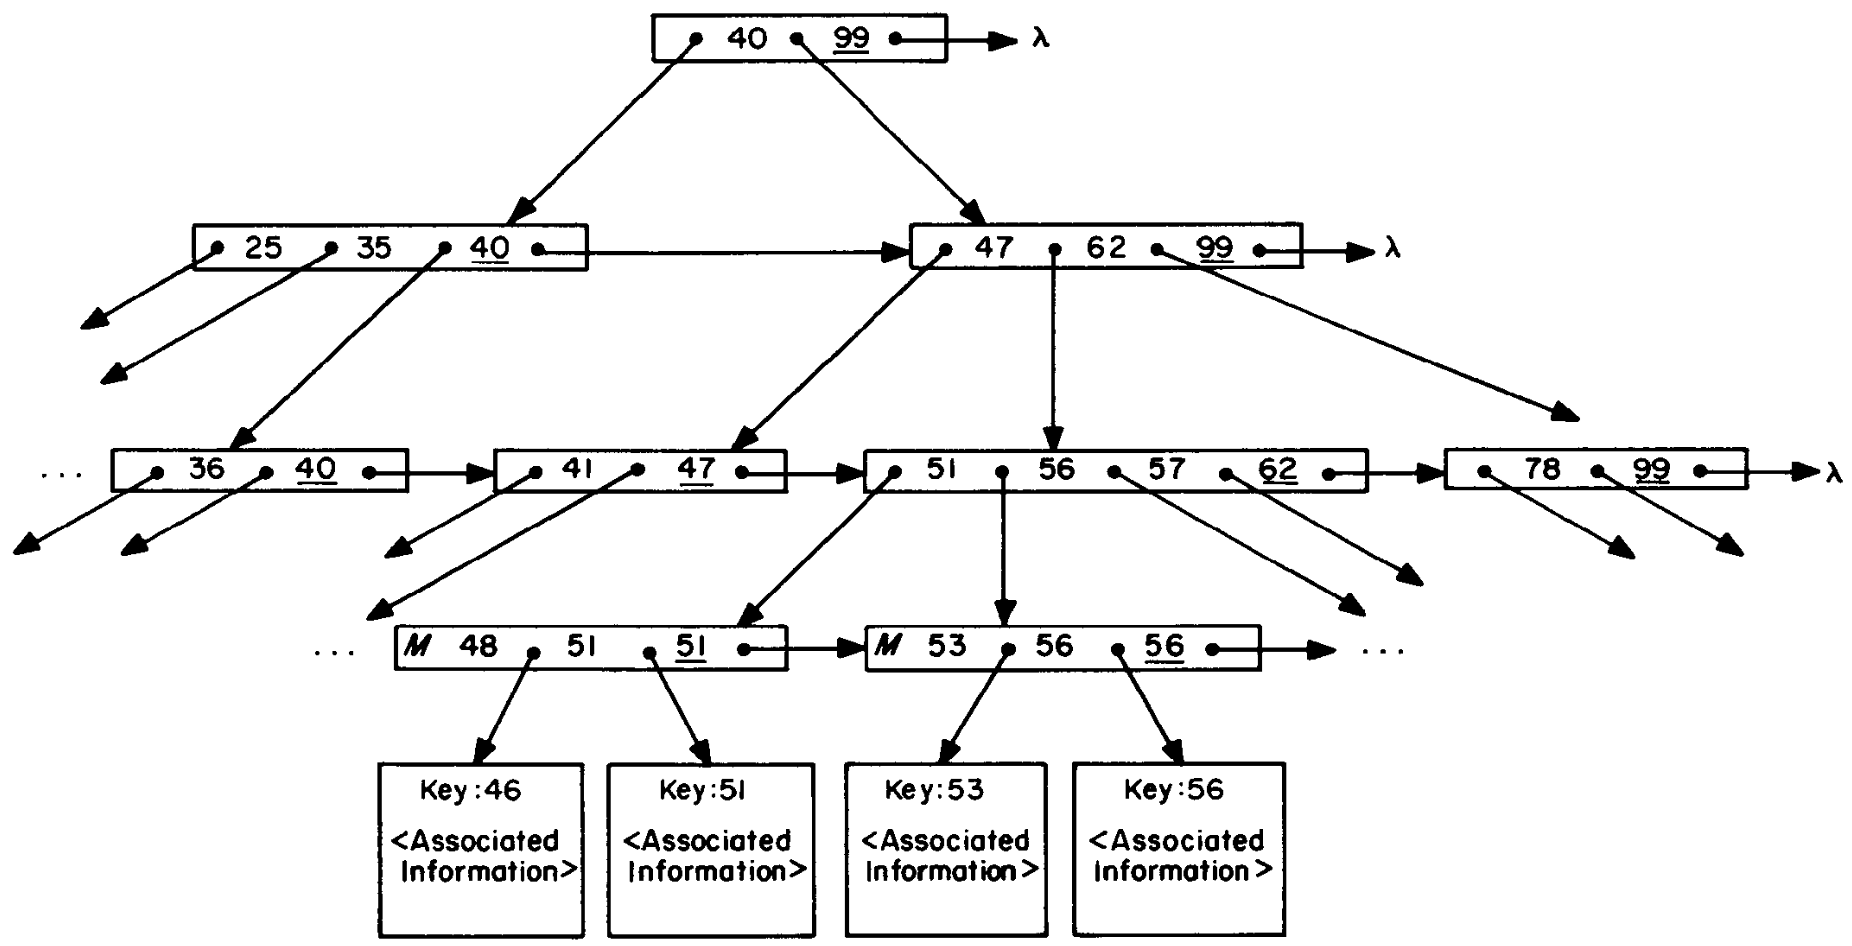
\includegraphics[width=\textwidth]{asset/blink_tree.png}
  \vspace{-1em}
  \caption{A $\text{B}^{\text{link}}$ tree}
  \label{fig:blink_tree}
\end{figure}

The type definition of the $\text{B}^{\text{link}}$ tree in Flix is as follows:
\begin{minted}{text}
enum BLinkTree[k: Type, v: Type, r: Region](Region[r], Ref[Node[k, v, r], r])
enum Node[k: Type, v: Type, r: Region] {
    case Inner(Int32, Ref[Int32, r], Array[k, r], Array[Node[k, v, r], r],
               Ref[Node[k, v, r], r], ReentrantReadWriteLock[r])
    case  Leaf(Int32, Ref[Int32, r], Array[k, r], Array[v, r],
               Ref[Node[k, v, r], r], ReentrantReadWriteLock[r])
    case Empty
}
\end{minted}

The node structure is similar to that of the B+ tree, with the addition of the high key, stored in the last element of the key array, the link, and the lock. The original paper uses a simple mutex lock because in their setting, a node is stored as a block in the disk. Reading a block is an atomic operation so there is no locking involved in the \texttt{get} method. It is only when then intension of reading the block is to update it that the lock is acquired. In our setting, we need to read-write locks because the nodes are stored in memory and when reading the fields in a node, we need to make sure that these fileds are not being modified at the same time by another thread. The extra ineteger represent the level of the node in the tree. Leaf nodes are at level 0, and the level increases as we go up the tree. Once a node is created, the level is fixed and will not change. Level is needed here to deal with the case that Lehman and Yao did not discuss, that is, when the root node is concurrently split by other threads. We will discuss this in section \ref{sec:blink-insert}.

\section{Search in $\text{B}^{\text{link}}$ Trees}
\label{sec:blink-search}

To search for a value $k$ in the tree, the search process begins at the root and proceeds by comparing $k$ with the keys in each node in a path down the tree. At each node, we first acquire the read lock and then examine the keys and high key. If $k$ is greater than the high key, we follow the link to the right sibling, unlock the current node, and repeat searching in the sibling. Otherwise, we examine the key array to find the index of the first key that is greater than or equal to $k$. Then we use the index to get the child node to follow. We unlock the current node, push it the stack, and repeat the search in the child node until we reach a leaf node.

The details of the search function is shown in algorithm \ref{alg:blink-search}, following the same naming convention in \ref{alg:bplus-insert}. Note how the high key is used to determine if we need to follow the link to the right sibling. In the descending function, even if we have found the correct child to follow at some level $i + 1$, when we examine that child node at level $i$, it is still possible that it has been split by another thread, and the key we are looking for is moved to the right.

Locking is involved in the function \texttt{searchInner} and \texttt{searchLeaf}. The difference is that in \texttt{searchInner}, when we have finished searching the current level and have obtained the correct child node to follow, we release the lock as we will then proceed to the next level. In \texttt{searchLeaf}, when the function returns, the lock is still held, as the node needs to be examined further depending on if we are only reading or doing insertion.

\begin{algorithm}[h]
  \caption{Search in $\text{B}^{\text{link}}$ Tree}\label{alg:blink-search}
  \begin{algorithmic}[1] % The number in square brackets specifies the line numbering
    \Function {get}{k, t}
    \State $root \gets \text{root}(t)$
    \State $leaf, stack \gets \text{descendToLeaf}(k, root, [])$
    \State $leaf', i \gets \text{searchLeaf}(k, leaf, \text{false})$
    \If {$i = \text{num}(keys)$ or $k \neq keys[i]$}
    \State release read lock of $leaf'$
    \State \Return None
    \Else
    \State $v \gets vals[i]$
    \State release read lock of $leaf'$
    \State \Return Some($v$)
    \EndIf
    \EndFunction
    \Function {descendToLeaf}{k, node, stack}
    \If {$node$ is leaf}
    \State \Return $node, stack$
    \Else
    \State $child, stack' \gets \text{searchInner}(k, node, stack)$
    \State \Return \text{descendToLeaf}$(k, child, stack')$
    \EndIf
    \EndFunction
    \Function {searchInner}{k, node, stack}
    \State acquire read lock of $node$
    \If {needToGoRight(k, node)}
    \State $sibling \gets \text{link}(node)$
    \State release read lock of $node$
    \State \Return \text{searchInner}(k, sibling, stack)
    \Else
    \State $i \gets \text{findFirstGreaterOrEqual}(k, keys)$
    \State $child \gets vals[i]$
    \State release read lock of $node$
    \State \Return $child$, $node :: stack$
    \EndIf
    \EndFunction
    \Function {searchLeaf}{k, node, isWriting}
    \State acquire read or write lock depending on $isWriting$
    \If {needToGoRight(k, node)}
    \State $sibling \gets \text{link}(node)$
    \State release read or write lock depending on $isWriting$
    \State \Return \text{searchInner}$(k, sibling, isWriting)$
    \Else
    \State $i \gets \text{findFirstGreaterOrEqual}(k, keys)$
    \State \Return $node, i$
    \EndIf
    \EndFunction
    \Function {needToGoRight}{k, node}
    \State \Return link($node$) $\neq$ null $\wedge$ $k > \text{high key}(node)$
    \EndFunction
  \end{algorithmic}
\end{algorithm}

\section{Insertion in $\text{B}^{\text{link}}$ Trees}
\label{sec:blink-insert}

To insert a key-value pair, we first perform operations similar to that for searching. Beginning at the root, we scan down the tree to the leaf node that should contain the key, keeping track of the rightmost node that we examined at each level in a stack.

The insertion of the key-value pair into the leaf node may necessitate splitting the node. In this case, we split the node as what we have seen in the B+ tree, with the addition of changing the high key. The high key of the new node is set to the high key of the old node, and the high key of the old node is set to the last key that remains in the old node after splitting, which is then pushed up to the parent node recoreded in the stack. The parent node, too, may need to be split. If so, we backtrack up the tree, splitting nodes and inserting new pointers into their parents. In all cases, we lock a node before modifying it. Just as what we discussed in the insertion algorithm of the B+ tree, the splitting of the inner node and the leaf node slightly differs. When splitting the leaf node, the high key is pushed up to the parent, while when splitting the inner node, it is the middle key which neither remains in the old node nor be put in the new node that is pushed up to the parent.

The details of the insertion algorithm is shown in algorithm \ref{alg:blink-insert}, again following the same naming convention in \ref{alg:bplus-insert}, where $keys$, $vals$, and $level$ are used to represent the key array, value array, and the level of the node that is currently examined in the context, i.e. $node'$.

\begin{algorithm}[h]
  \caption{Insert in $\text{B}^{\text{link}}$ Tree}\label{alg:blink-insert}
  \begin{algorithmic}[1] % The number in square brackets specifies the line numbering
    \Function {put}{k, v, t}
    \State $root \gets \text{root}(t)$
    \State $leaf, stack \gets \text{descendToLeaf}(k, root, [])$
    \State insertLeaf($k, v, leaf, stack, root$)
    \EndFunction

    \Function {insertLeaf}{k, v, node, stack, root}
    \State $node', i \gets \text{searchLeaf}(k, node', \text{true})$
    \If {$i < \text{num}(keys)$ and $k = keys[i]$}
    \State $vals[i] \gets v$
    \State release write lock of $node'$
    \Else
    \State $k', v' \gets \text{insert k and v into the key and value array}$
    \If {$k'$ and $v'$ are null}
    \State increase the number of keys in the $node'$ by 1
    \State release write lock of $node'$
    \Else
    \State $newNode, upKey \gets \text{splitLeaf}(node', k', v')$
    \State release write lock of $node'$
    \If {$stack$ is empty}
    \If {level($root$) $ = level$}
    \State $newRoot \gets \text{create a new inner node}$
    \State put $upKey$, $node'$, and $newNode$ in $newRoot$
    \State $root \gets newRoot$
    \Else
    \State redescend($upKey$, $newNode$, $level$, $root$)
    \EndIf
    \Else
    \State $parent \gets \text{pop}(stack)$
    \State insertInner($upKey$, $newNode$, $parent$, $stack$, $root$)
    \EndIf
    \EndIf
    \EndIf
    \EndFunction

    \Function {insertInner}{k, n, node, stack, root}
    \State same as insertLeaf, with the function of splitLeaf replaced by splitInner
    \EndFunction

    \Function {redescend}{k, n, toLevel, root}
    \State $node, stack \gets \text{descendToLevel}(k, toLevel, root, [])$
    \State insertInner($k$, $n$, $node$, $stack$, $root$)
    \EndFunction

    \Function {descendToLevel}{k, toLevel, node, stack}
    \If {level($node$) $ = toLevel + 1$}
    \State \Return $node$, $stack$
    \Else
    \State $child, stack' \gets \text{searchInner}(k, node, stack)$
    \State \Return \text{descendToLevel}($k$, $toLevel$, $child$, $stack'$)
    \EndIf
    \EndFunction
  \end{algorithmic}
\end{algorithm}

We mentioned before that unlike the original paper, for the rightmost node at each level, the high key is set to $+\infty$ instead of the actual largest key in this subtree. This makes splitting the rightmost leaf node easier. When the rightmost leaf is split, we can always safely set the high key of the new node to that of the old node, which is $+\infty$, regardless of if we have inserted a key that is greater than all existing keys. This makes spiltting the rightmost node consistent with splitting other nodes.

We also mentioned that Lehman and Yao fail to discuss what must happen when the root node becomes full and must be split. When an inserter recurses up the tree, it is possible it has recursed up to the root but the root level has been split by other threads and a new root has been created. In this case the stack it made while descending does not help for finding the correct parents anymore. We adopt the solution from PostgreSQL. PostgreSQL has adpoted $\text{B}^{\text{link}}$ trees as base for its index structure. Their solution is that when this happens, we re-descending the tree until we reach the level one above the old root. Typically the re-descending only needs to examine one level of nodes, because in most cases, if the old root level has been split, there will be enough space for insertion and re-descending is not needed. It is rare that the root level is split and is quickly filled up again by other threads. In this case, the re-descending is needed. But it is highly unlikely that even the new root level is split and filled up.

This locking scheme is efficient in that only a constant number of nodes are locked at any time. The original paper couples locks as part of moving right when relocating a child node's downlink during an ascent of the tree.  This is the only point where it has to simultaneously hold three locks (a lock on the child, the original parent, and the original parent's right sibling). However, in our implementation, an inserter nevers couples any locks, neither between the child and the parent, nor between siblings. This means that only one lock is held at any time. We will not give a rigorous proof of the correctness here but we argue that as long as we always obtain the correct pointer to follow from the current node when the current node is locked, and we always lock the node the pointer points to before accessing its fields, the implementation is correct.

%%%%%%%%%%%%%%%%%%%%%%%%%%%%%%%%%%%%%%%%%%%%%%%%%%%%%%%%%%%%%%%%%%%%%%%

\chapter{Evaluation}
\label{ch:evaluation}

In this chapter, we answer the following five research questions:

\begin{itemize}
  \item[\textbf{RQ0}] Does our implementation of the trees satisfy the asymptotic bound?
  \item[\textbf{RQ1}] Is insertion and range query in the B+ tree faster than in the built-in map that use red-black trees?
  \item[\textbf{RQ2}] Is insertion and range query in the $\text{B}^{\text{link}}$ tree faster than in the B+ tree and red-blakc tree?
  \item[\textbf{RQ3}] Is Datalog evaluation using B+ trees faster than using red-black trees?
  \item[\textbf{RQ4}] Is Datalog evaluation using $\text{B}^{\text{link}}$ trees faster than using B+ trees and red-black trees?
\end{itemize}

To answer the question 0 and 1, we do the following experiment.

\newpage
\newgeometry{top=1in, bottom=1in, left=0.8in, right=0.8in}
\begin{figure}[htbp]
  \centering
  \begin{minipage}[b]{0.49\textwidth}
    \centering
    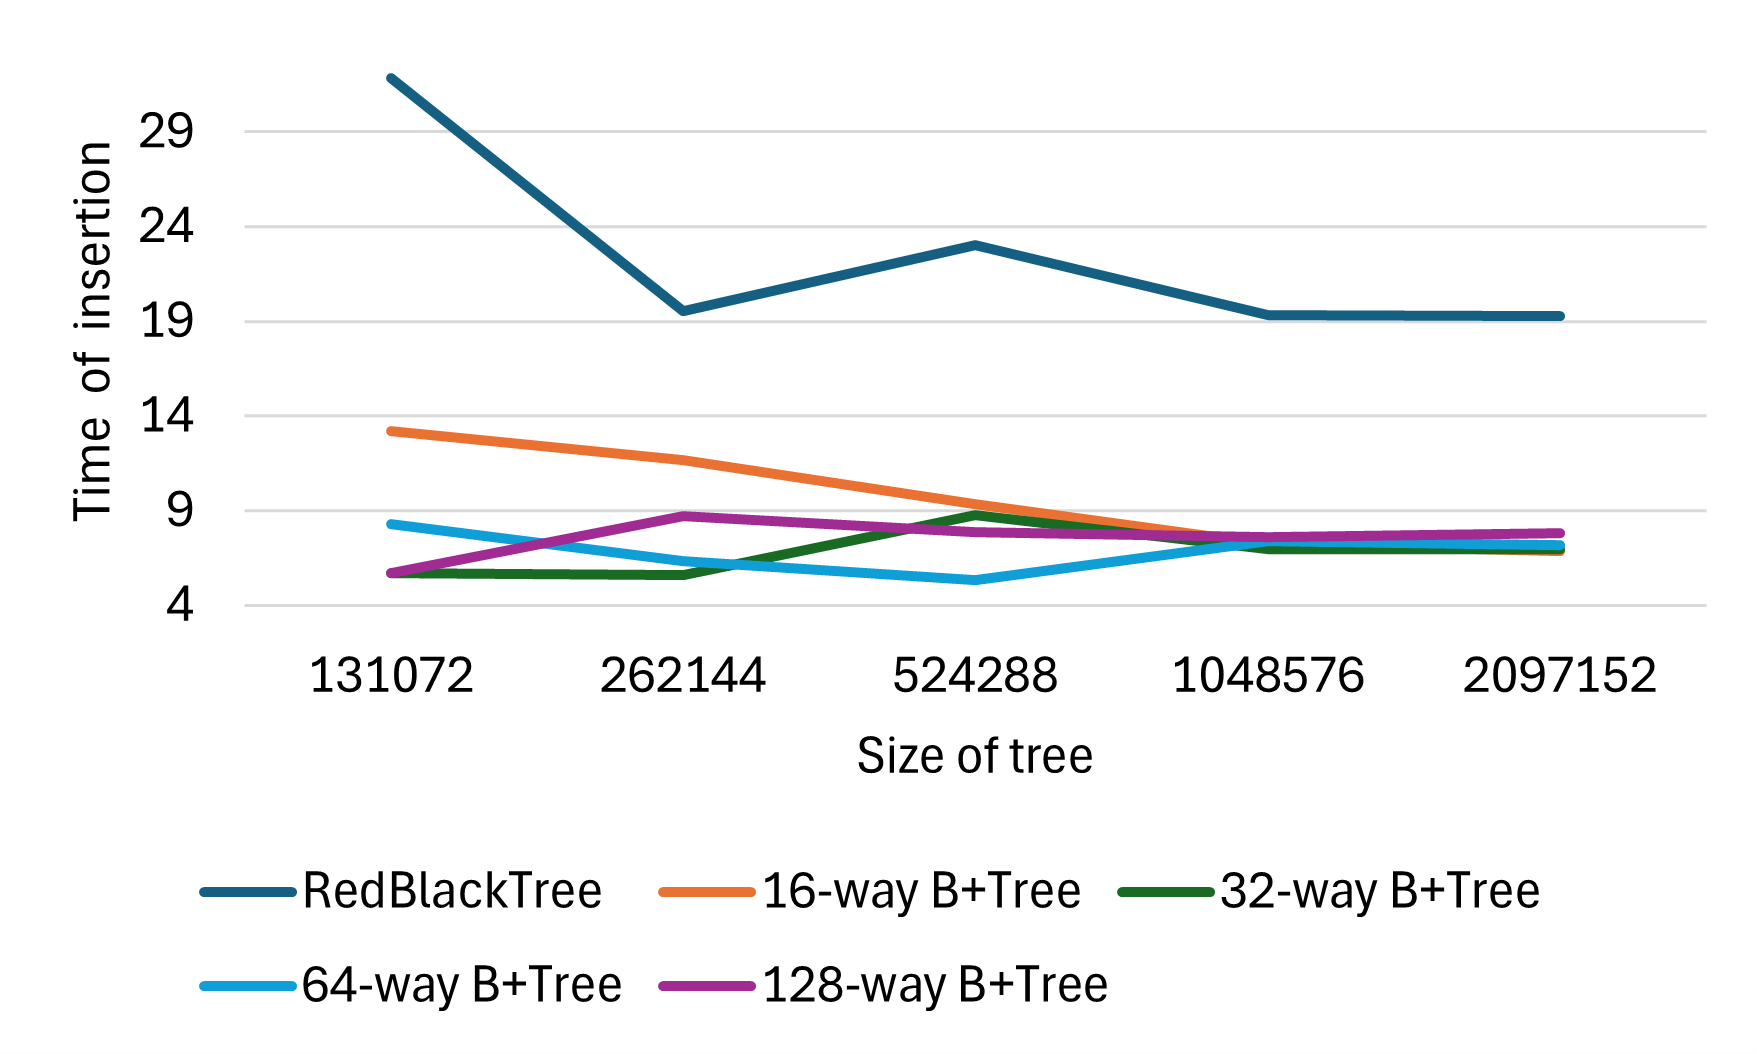
\includegraphics[width=\textwidth]{asset/insert.png}
    \captionsetup{width=0.9\textwidth}
    \caption{Time of inserting 1 value in Red-Black Tree and B+Trees}
    \label{fig:insert_BPlusTree}
  \end{minipage}
  \begin{minipage}[b]{0.49\textwidth}
    \centering
    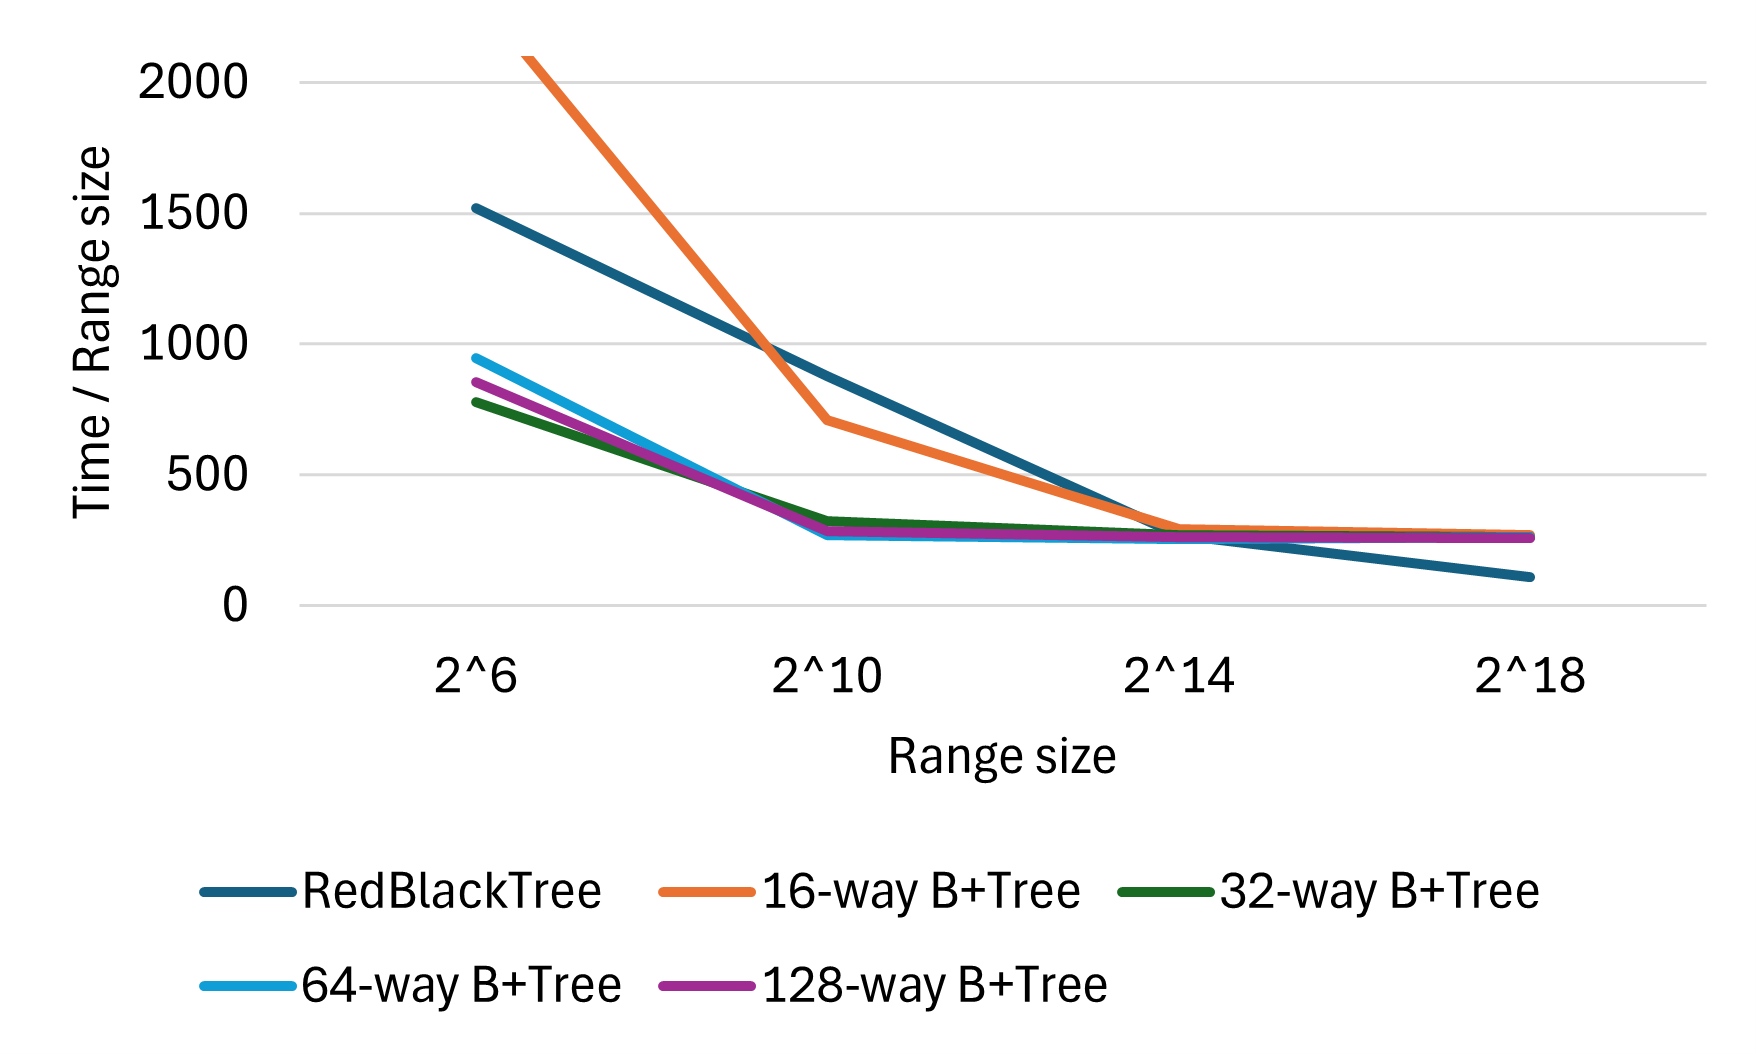
\includegraphics[width=\textwidth]{asset/range_query.png}
    \captionsetup{width=0.9\textwidth}
    \caption{Time of range query in Red-Black Tree and B+Trees containing $2^{20}$ keys}
    \label{fig:rq_BPlusTree}
  \end{minipage}

  \vspace{0.5cm}

  % \caption{Overall caption for the figure}
  % \label{fig:overall}
\end{figure}
\restoregeometry

%%%%%%%%%%%%%%%%%%%%%%%%%%%%%%%%%%%%%%%%%%%%%%%%%%%%%%%%%%%%%%%%%%%%%%%

\chapter{Future Work}
\label{ch:future_work}

\chapter{Conclusion}
\label{ch:conclusion}

\todo{Conclude on the problem statement from the introduction}

%%%%%%%%%%%%%%%%%%%%%%%%%%%%%%%%%%%%%%%%%%%%%%%%%%%%%%%%%%%%%%%%%%%%%%%

\cleardoublepage
\addcontentsline{toc}{chapter}{Bibliography}
\bibliographystyle{plain}
\bibliography{refs}

%%%%%%%%%%%%%%%%%%%%%%%%%%%%%%%%%%%%%%%%%%%%%%%%%%%%%%%%%%%%%%%%%%%%%%%

\cleardoublepage
\appendix
\chapter{The Technical Details}

\todo{\dots}

\end{document}
